\documentclass[tikz,border=5pt]{standalone}
\usepackage{amsmath}
\usepackage{braket}
\usetikzlibrary{arrows.meta, shapes.misc, positioning, backgrounds}

\begin{document}
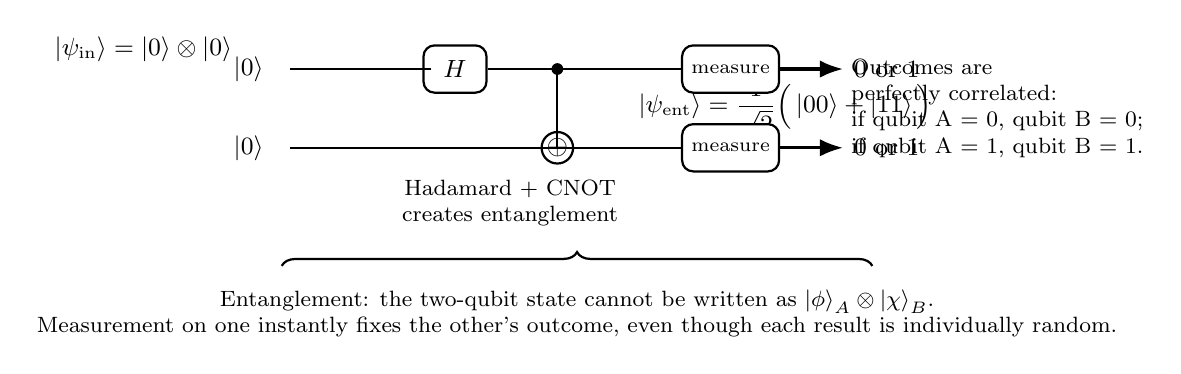
\begin{tikzpicture}[
   thick,
   wire/.style={thick},
   gate/.style={draw, rounded corners, minimum width=0.8cm, minimum height=0.6cm, font=\small, fill=white},
   ctrl/.style={fill=black, circle, inner sep=1.5pt},
   target/.style={draw, circle, inner sep=0pt, minimum width=0.4cm},
   measure/.style={draw, rounded corners, minimum width=0.9cm, minimum height=0.6cm, font=\scriptsize, fill=white},
   amp/.style={-Latex, very thick},
   note/.style={font=\small},
   outcome/.style={font=\small, align=center},
   corr/.style={font=\footnotesize},
]

%%%% 1. LEFT: Initial product state %%%%

\node[note, anchor=east] (psi0label) at (-0.4,0.75)
{$\displaystyle \ket{\psi_\text{in}} = \ket{0}\otimes\ket{0}$};

% Input kets (two wires)
\node[note, anchor=east] (q0in) at (0,0.5) {$\ket{0}$};
\node[note, anchor=east] (q1in) at (0,-0.5) {$\ket{0}$};

% Horizontal wires (input region to circuit region)
\draw[wire] (0.2,0.5) -- (2.0,0.5);
\draw[wire] (0.2,-0.5) -- (2.0,-0.5);

%%%% 2. CIRCUIT: H on top, then CNOT %%%%

% Hadamard gate on first qubit
\node[gate] (Hgate) at (2.3,0.5) {$H$};

\draw[wire] (2.0,0.5) -- (Hgate.west);
\draw[wire] (Hgate.east) -- (3.2,0.5);

% Vertical line for CNOT control-target
\draw[wire] (3.6,0.5) -- (3.6,-0.5);

% Control dot on top wire
\node[ctrl] (ctrl) at (3.6,0.5) {};

% Target ⊕ on bottom wire
\node[target] (targ) at (3.6,-0.5) {$\oplus$};

% extend wires to the right of CNOT
\draw[wire] (3.2,0.5) -- (4.2,0.5);
\draw[wire] (2.0,-0.5) -- (4.2,-0.5);

% Label under circuit: "Entangling operation"
\node[font=\footnotesize, align=center] at (3.0,-1.2)
{Hadamard + CNOT\\creates entanglement};

%%%% 3. STATE AFTER CIRCUIT %%%%

\node[note, anchor=west] (psiBell) at (4.5,0.0)
{$\displaystyle
\ket{\psi_\text{ent}} =
\frac{1}{\sqrt{2}}\Big(\ket{00}+\ket{11}\Big)
$};

%%%% 4. MEASUREMENT BOXES %%%%

% Measurement boxes on each qubit
\node[measure] (M0) at (5.8,0.5) {measure};
\node[measure] (M1) at (5.8,-0.5) {measure};

% wires into measurement
\draw[wire] (4.2,0.5) -- (M0.west);
\draw[wire] (4.2,-0.5) -- (M1.west);

% classical arrows out
\draw[amp] (M0.east) -- ++(0.8,0.0) node[outcome, anchor=west]
{$0$ or $1$};
\draw[amp] (M1.east) -- ++(0.8,0.0) node[outcome, anchor=west]
{$0$ or $1$};

% Correlation annotation
\node[corr, align=left, anchor=west] at (7.2,0.0)
{Outcomes are\\perfectly correlated:\\
if qubit A = 0, qubit B = 0;\\
if qubit A = 1, qubit B = 1.};

%%%% 5. BIG BRACE + TEXT EXPLANATION %%%%

% Decorative brace under entire figure
\draw[decorate, decoration={brace, amplitude=5pt}]
 (0.1,-2.0) -- (7.6,-2.0)
 node[midway, yshift=-0.6cm, align=center, font=\footnotesize]
 {Entanglement: the two-qubit state cannot be written
  as $\ket{\phi}_A \otimes \ket{\chi}_B$.\\
  Measurement on one instantly fixes the other's outcome,
  even though each result is individually random.};

\end{tikzpicture}
\end{document}
